\section{Durchführung}
\label{sec:Durchführung}
Für den Versuch wird der in \autoref{fig:skizze} dargestellte Aufbau verwendet. Darin wird das Zählrohr über eine Spannungsquelle
versorgt. Wenn ein Impuls gemessen wird, fließt die gesammelte Ladung über einen Widerstand ab und wird durch einen Kondensator
ausgekoppelt. Der Impuls wird dann entweder verstärkt an einen Zähler geleitet und dort gezählt oder an einen Oszillographen, an dem
in einem späteren Versuchsteil die Totzeit abgelesen werden kann. Bei diesem Versuch wird das Element $\ce{^{204}Tl}$ verwendet. Dieses
wird vor dem Geiger-Müller-Zählrohr in einer Apparatur fixiert.
\begin{figure}
    \centering
    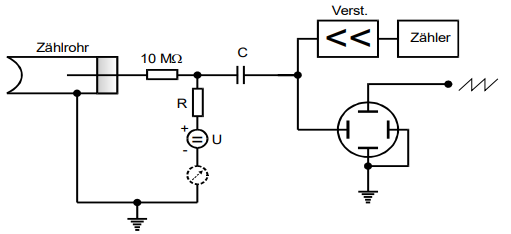
\includegraphics[width=0.9\textwidth]{content/skizze.png}
    \caption{Skizze des Versuchaufbaues.}
    \label{fig:skizze}
\end{figure}

Zunächst wird die Charakteristik des Geiger-Müller-Zählrohres untersucht. Dazu wird die Zählrate des Zählrohres bei verschiedenen
angelegten Spannungen, im Bereich von 320 V bis 680 V in 20 V-Schritten, gemessen. Zusätzlich wird die Stromstärke, wenn möglich, am
Zählrohr abgelesen und ebenfalls mit den zugehörigen Spannungen notiert. Dies ist erforderlich um die vom Zählrohr pro Teilchen
freigesetzte Ladungsmenge zu bestimmen.

Im zweiten Versuchsteil wird die Totzeit des Zählrohres bestimmt. Dabei muss dafür gesorgt sein, dass eine
hohe Strahlintensität in das Zählrohr eintritt. Hier wird eine Spannung von 500 V verwendet.
Die Bestimmung wird über zwei verschiedene Methoden durchgeführt. 
Zum Einen wird die Totzeit mithilfe des Oszillographen bestimmt. Wenn die Zeitablenkung durch die Anstiegsflanke des Zählrohres
getriggert wird, lässt sich auf dem Schirm die Totzeit ablesen. Zur Verbesserung des Messergebnisses wird der Bildschirm einige Zeit
abgefilmt um das Ablesen von diesem zu erleichtern. Zum Anderen wird die sogenannte Zwei-Quellen-Methode verwendet. Diese erfolgt wie
in der Theorie beschriebn, wobei hier 
über einen Zeitraum von 60 s gemessen wird. Die zweite Quelle ist ebenfalls $\ce{^{204}Tl}$.

